\SetVertexNormal[Shape      = circle,
                 FillColor  = orange,
                 LineWidth  = 1.5pt]
\SetUpEdge[lw         = 1pt,
           color      = black,
           labelcolor = white,
           labeltext  = red,
           labelstyle = {sloped,draw,text=blue}]
\begin{center}
\begin{tikzpicture}
   \Vertex[x=-1,y=0]{S}
   \Vertex[x=11 ,y=0]{T}
   \Vertex[x=5,y=0]{Z}
   \Vertex[x=1 ,y=1]{A}
   \Vertex[x=3 ,y=2]{B}
   \Vertex[x=5,y=2]{C}
   \Vertex[x=7 ,y=2]{D}
   \Vertex[x=9 ,y=1]{E}
   \Edge[label = $13$](S)(Z)
   \Edge[label = $11$](Z)(T)
   \Edge[label = $2$,color=gray](S)(A)
   \Edge[label = $3$,color=gray](A)(B)
   \Edge[label = $4$,color=gray](B)(C)
   \Edge[label = $5$,color=gray](C)(D)
   \Edge[label = $6$,color=gray](D)(E)
   \Edge[label = $7$,color=gray](E)(T)
   \tikzset{EdgeStyle/.append style = {bend left}}
\end{tikzpicture}\\
{\small El camino superior tiene longitud 27, mientras que el inferior 24.}
\end{center}